\chapter{Nodos}
\section{Introducción}
Un diagrama de nodos o de despliegue muestra las relaciones físicas de los nodos que la componen, además de cómo se reparten los nodos en cada nodo. Algunas de las ventajas de el uso de este tipo  de diagramas es la visión holística que se puede tener del proyecto, ya que muestra la relación y distribución de la parte de hardware y software. El problema de esto es que al ser tan general no se pueden vislumbrar algunos detalles que si se pueden ver en otro tipo de diagramas.
\section{Marco Teórico}
Un diagrama de despliegue se compone de:
\begin{itemize}
\item Nodo: Es un elemento de hardware o software que se muestra como una caja en tres dimensiones.
\begin{figure}[H]
	\centering
	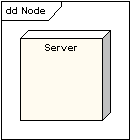
\includegraphics[width=1\linewidth]{diseno/nodos/imgs/1}
	\caption{Nodo. Imagen tomada de internet}
	\label{fig:gantt}
\end{figure}

\item Instancia de nodo: Una instancia se puede distinguir de un nodo por el hecho de que su nombre esta subrayado y tiene dos puntos antes del tipo de nodo base. 
\begin{figure}[H]
	\centering
	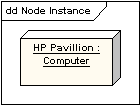
\includegraphics[width=1\linewidth]{diseno/nodos/imgs/2}
	\caption{Instancia de un nodo. Imagen tomada de internet}
	\label{fig:gantt}
\end{figure}

\item Estereotipo de nodo: Estereotipos estándar se proveen para los nodos, nombrados «cdrom», «cd-rom», «computer», «disk array», «pc», «pc client», «pc server», «secure», «server», «storage», «unix server», «user pc». Estos mostrarán un icono apropiado en la esquina derecha arriba del símbolo nodo.

\begin{figure}[H]
	\centering
	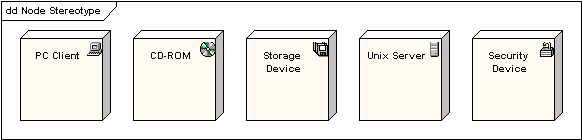
\includegraphics[width=1\linewidth]{diseno/nodos/imgs/3}
	\caption{Estereotipo de Nodo. Imagen tomada de internet}
	\label{fig:gantt}
\end{figure}

\item Artefacto: Un artefacto es un producto del proceso de desarrollo de software, que puede incluir los modelos del proceso como los casos de uso, los modelos de diseño, etc.

\begin{figure}[H]
	\centering
	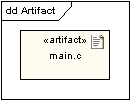
\includegraphics[width=1\linewidth]{diseno/nodos/imgs/4}
	\caption{Artefacto. Imagen tomada de internet}
	\label{fig:gantt}
\end{figure}

\end{itemize}

\section{Diagrama de nodos}
